\begin{infocard}{Suma de los ángulos internos de un triángulo}
    \begin{figure}[H]
        \centering
        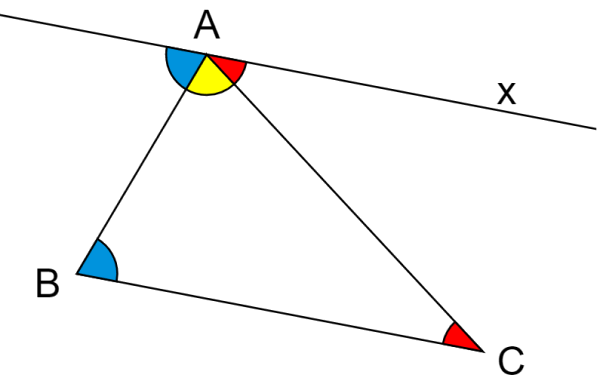
\includegraphics[width=0.9\linewidth]{../images/angulos-internos-de-un-triangulo.png}
    \end{figure}
    La suma de los ángulos internos de un triángulo es:
    {\large\[\angle {\color{colorrds}B} + \angle {\color{red}C} + \angle {\color{yellow}A}=180^\circ\]}
\end{infocard}